\documentclass[11pt]{article}
\usepackage[letterpaper,margin=1in]{geometry}
\usepackage[T1]{fontenc}
\usepackage{mathptmx}
\usepackage{amsmath,amssymb}
\usepackage{graphicx}
\usepackage{booktabs}
\usepackage[font=small,labelfont=bf]{caption}
\usepackage[numbers,sort&compress]{natbib}
\usepackage{xcolor}
\usepackage{microtype}
\usepackage{authblk}
\usepackage[colorlinks=true,linkcolor=blue!50!black,citecolor=blue!50!black,urlcolor=blue!50!black]{hyperref}
\setlength{\emergencystretch}{3em}
\renewcommand{\baselinestretch}{1.12}
\newcommand{\LIO}{\texorpdfstring{LaInO$_3$}{LaInO3}}
\newcommand{\BSO}{\texorpdfstring{BaSnO$_3$}{BaSnO3}}
\newcommand{\ntot}{n_\mathrm{tot}}
\newcommand{\xmax}{x_\mathrm{max}}
\makeatletter\newcommand{\inputrows}[1]{\@@input #1 }\makeatother

\title{Why the Hall density of electrolyte-gated \LIO/\BSO\ falls on cooling: subband transport, the place of the compensating charge, and a resistance upturn too large for weak localization}
\author{Gracen Ownby}
\affil{University of Oklahoma, Norman, Oklahoma, USA}
\date{\small 14 October 2026}

\begin{document}
\maketitle

\begin{abstract}
In the electrolyte-gated \LIO/\BSO\ two-dimensional electron gas of Lee \emph{et al.}, the ions are frozen below 220~K, so each gate voltage fixes the positive charge; yet at 8~V the Hall density falls from $1.08\times10^{14}$~cm$^{-2}$ at 150~K to $6.5\times10^{13}$~cm$^{-2}$ at 2~K while the Hall mobility rises to 1990~cm$^2$/Vs. We analyse the published data with a self-consistent Schr\"odinger--Poisson model of the interface and a multisubband transport calculation (static multisubband screening, coupled Boltzmann equations, Hall response of parallel subbands at finite field). Three results follow. First, below 50~K the sheet resistance rises by 10, 19 and 27\% at 5, 7 and 8~V, in the resistance data and in the Hall data alike; at $k_Fl\approx60$--530 this is 5--170 times the logarithmic conductance change that weak localization and electron--electron interaction can produce, so the upturn is not a quantum correction, and the Hall density falls in proportion to the conductance while the Hall mobility stays within 5\%. Second, a Hall density below the electron density needs subbands of unequal mobility. A strongly compensated \BSO\ layer has a single occupied subband up to $6.5\times10^{13}$~cm$^{-2}$ and cannot produce the drops of 10--15\% at 4--5~V; at 7--8~V it would need upper subbands 7--19 times more mobile than the ground subband and a Hall resistance bent by 14--30\% over 0--7~T, which the reported linear Hall resistance excludes. Clean \BSO, with two or three occupied subbands, needs upper subbands 1.5--1.6 (50~K) and 2.2--2.4 (2~K) times more mobile at 4--5~V, with bending below 1\%, and 2.7--6.6 times at 7--8~V, with 3--9\% bending. Coulomb scattering by the positive charge that balances the gated electrons, next to the interface where electrostatics requires it, makes the upper subbands 1.6--2.1 times more mobile whatever its distance and charge, accounting for the 50~K data at 4--5~V and for about half of the effect at 7--8~V. Third, the measured conductance bounds how close that charge can be: at 8~V, random point charges must lie at least 5.5~\AA\ (singly charged) or 8.4~\AA\ (doubly charged) from the interface, while electrostatics allows at most 4.3--7.9~\AA\ for clean \BSO\ and 1.8--2.8~\AA\ for compensated \BSO. The data thus point to clean \BSO\ with singly charged, or spatially correlated, positive charge in the first one or two \LIO\ unit cells. The remaining drop below 50~K requires either a ground-subband mobility that halves on cooling from 100 to 2~K, which no static scatterer gives, or the loss of about $1.7\times10^{13}$~cm$^{-2}$ mobile electrons at fixed positive charge; the curvature of the Hall resistance at 2~K decides between them. In both readings the conductivity mobility per electron at 8~V and 2~K is 1200~cm$^2$/Vs.
\end{abstract}

\section{Introduction}
The two-dimensional electron gas (2DEG) at the polar interface between \LIO\ and \BSO\ combines a polarization-induced density of a few $10^{13}$~cm$^{-2}$ with the high mobility of \BSO\ \cite{Kim2016LIO,Kim2019LIO,Aggoune2021}. Lee \emph{et al.} gated it with an ionic liquid on a 5~nm \LIO\ cap over 110~nm of \BSO\ grown by molecular-beam epitaxy on MgO \cite{Lee2024LIO}. Each gate voltage $V_{GS}$ was applied at 220~K, where the liquid is still mobile, and the sample was then cooled with the ions frozen. Their Fig.~3 reports the sheet resistance from 2 to 220~K and the Hall density $n_H$ and Hall mobility $\mu_H$ at 2, 10, 50, 100 and 150~K for $V_{GS}=0$--8~V. At 8~V the Hall density reaches $1.08\times10^{14}$~cm$^{-2}$ at 150~K and the Hall mobility 1990~cm$^2$/Vs at 2~K, the highest reported for a \BSO-based system. Two features of these data are not explained in Ref.~\cite{Lee2024LIO}: at high bias the Hall density falls on cooling (``not well understood at this point''), and the sheet resistance rises slowly at low temperature, ``almost in the shape of $\log T$'', which is attributed to weak localization.

The first feature is puzzling because the positive charge is fixed. Electrons cannot disappear at fixed positive charge, so either some of them stop being counted by the Hall measurement or they move into states that do not conduct. In a companion study we showed that the positive charge must sit within about one \LIO\ unit cell of the interface to keep electrons out of the cap at these densities \cite{OwnbyMAT02}; there we left the drop on cooling open. Here we analyse it. The Hall density of several parallel channels, $n_H=(\sum_in_i\mu_i)^2/\sum_in_i\mu_i^2$, equals the electron density only if all channels have the same mobility, and at $10^{14}$~cm$^{-2}$ the interface has two or three occupied subbands. The question is therefore whether the subbands of this interface differ enough in mobility, for what reason, and whether the answer is compatible with the other published observations: the linear Hall resistance up to 7~T, the sheet resistance, and the location of the positive charge required by electrostatics.

We find that the upturn is two orders of magnitude too large for weak localization; that the strongly compensated \BSO\ assumed in earlier work on this interface is incompatible with the Hall data of this sample; that Coulomb scattering by the positive charge next to the interface, which electrostatics requires, makes the upper subbands about twice as mobile as the ground subband and explains a large part of the drop; that the measured conductance in turn limits how close that charge can be, leaving a window of a few \aa ngstr\"oms at 8~V; and that the rest of the drop below 50~K requires either a ground-subband scattering that grows on cooling or carrier loss, which the field dependence of the Hall resistance would distinguish.

\section{Data}\label{sec:data}
We digitized Fig.~3b of Ref.~\cite{Lee2024LIO} (Hall density and mobility, five temperatures, nine gate voltages) and Fig.~3a (sheet resistance) for 5--8~V, where the curves are separated; for 0--4~V the resistance curves overlap and are not used. The 6~V Hall markers at 2 and 10~K are hidden behind the 7~V markers and are not used. The digitization is accurate to a few per cent on the logarithmic axes; the 2~K, 8~V values (Hall density $6.49\times10^{13}$~cm$^{-2}$, mobility 1985~cm$^2$/Vs) agree with the values quoted in the text of Ref.~\cite{Lee2024LIO} ($6.52\times10^{13}$~cm$^{-2}$, 1999~cm$^2$/Vs) to 0.7\%.

For parallel Drude channels the conductance is $\sigma=e\sum_in_i\mu_i=e\,n_H\mu_H$ exactly, so $R_s=1/(e\,n_H\mu_H)$ can be compared with the resistance of Fig.~3a. The two differ by a factor of 1.12--1.48 that grows with gate voltage, perhaps from the geometry used for $R_s$ or from different cool-downs; their temperature dependence agrees: between 50 and 2~K the resistance rises by 9.7, 18.5 and 26.8\% at 5, 7 and 8~V in Fig.~3a and by 9.8, 23.9 and 32.0\% in the Hall data (Fig.~\ref{fig:data}b). Only relative changes are used below, except in Sec.~\ref{sec:where}, where the Hall data set the conductance.

With the ions frozen, the electron density $\ntot$ at a given gate voltage is the same at all temperatures. Since $n_H\le\ntot$, the largest measured Hall density, at 150~K, is a lower bound on $\ntot$; we set $\ntot=n_H(150\ \mathrm{K})$, which assumes equal subband mobilities at 150~K, where phonon scattering dominates. With a larger $\ntot$ all required mobility differences grow. The Hall density at 2~K is then 90, 85, 74 and 60\% of $\ntot$ at 4, 5, 7 and 8~V (Fig.~\ref{fig:data}a). At 2--3~V the sheet resistance is 2.5--3~k$\Omega$, $k_Fl\approx10$, close to the metal--insulator crossover that Ref.~\cite{Lee2024LIO} places near 2~V; we concentrate on 4--8~V, where the 2DEG is a good metal.

\begin{figure}[t]
\centering
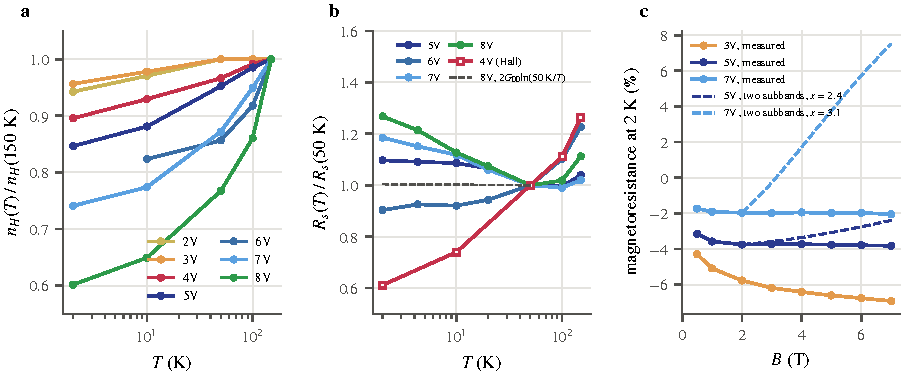
\includegraphics[width=\textwidth]{figures/fig1_data.pdf}
\caption{Data of Lee \emph{et al.} \cite{Lee2024LIO}, digitized. (a) Hall density relative to its 150~K value, with the gate charge frozen. (b) Sheet resistance relative to 50~K from Fig.~3a of Ref.~\cite{Lee2024LIO} (filled) and from $1/(e\,n_H\mu_H)$ (open); the rise above 150~K belongs to the range 150--220~K in which the liquid is not yet frozen. Dashed: the 8~V curve if the conductance fell by $2G_{00}\ln(50\,\mathrm{K}/T)$, about the largest that weak localization and the interaction correction give together.}
\label{fig:data}
\end{figure}

\section{Model}\label{sec:model}
\emph{Electrostatics and subbands.} The interface is described by the self-consistent Schr\"odinger--Poisson model of Refs.~\cite{OwnbyMAT01,OwnbyMAT02}, implemented in qwkit \cite{qwkit}: a Kane-nonparabolic conduction band of \BSO\ (mass $0.19\,m_0$, nonparabolicity 0.56~eV$^{-1}$, static permittivity 20), a 5~nm \LIO\ cap (offset 1.6~eV, mass $0.46\,m_0$, permittivity 24), deep acceptors in the \BSO\ depleting over a width set by Fermi-level pinning, and a fixed interface charge that gives $5\times10^{12}$~cm$^{-2}$ without gating. We consider strongly compensated \BSO\ ($N_A=5\times10^{19}$~cm$^{-3}$, as reported by Kim \emph{et al.} for pulsed-laser-deposited films \cite{Kim2019LIO}) and clean \BSO\ ($10^{18}$~cm$^{-3}$). The added positive charge is placed next to the interface (field-free cap), as Ref.~\cite{OwnbyMAT02} requires; by Gauss's law the \BSO\ side, and hence the subbands, do not depend on its exact place while the cap is empty. Ten subbands enter the self-consistency at 2~K on a 0.5~\AA\ grid.

In compensated \BSO\ the depletion field binds the 2DEG tightly, and the second subband is occupied only above $6.5\times10^{13}$~cm$^{-2}$; at $1.08\times10^{14}$~cm$^{-2}$ the ground subband holds 88\% of the electrons. In clean \BSO\ the second subband is occupied from about $1.5\times10^{13}$~cm$^{-2}$ and the ground subband holds 84, 81, 79 and 76\% at 4, 5, 7 and 8~V, with 3\% in a third subband at 8~V. We write $f_1$ for the ground-subband fraction.

\emph{Scattering.} At low temperature we compute the momentum relaxation times of all occupied subbands at the Fermi level from the coupled Boltzmann equations of Siggia and Kwok \cite{SiggiaKwok1970}, with the Born matrix elements of point charges $Ze$ at a distance $d$ from the interface,
\begin{equation}
V_{ij}(q)=\frac{Ze^2}{2\varepsilon_0\varepsilon q}\int\psi_i(z)\psi_j(z)\,e^{-q|z+d|}\,dz ,
\end{equation}
screened in the static random-phase approximation with the intrasubband Lindhard polarizabilities of all occupied subbands acting on intra- and intersubband elements alike \cite{SiggiaKwok1970,AFS1982}. The density-of-states mass at the Fermi level of each subband includes the nonparabolicity. The scatterers are (i) the positive charge added by gating, $\ntot+N_\mathrm{dep}-\sigma_P$, as random point charges with $Z=1$ or 2 (singly or doubly ionized donors, such as oxygen vacancies) in a plane $d=1$--48~\AA\ inside the cap, (ii) the ionized acceptors of the depletion layer, and (iii) charged threading dislocations, lines along $z$ with one electron per 4.116~\AA\ that scatter only within a subband \cite{Jena2000}, at densities $10^{10}$--$10^{11}$~cm$^{-2}$. The calculation reproduces an independent quadrature of the single-subband integral to $10^{-3}$, and the subband mobilities change by less than 0.1\% between 32 and 128 angles and a 0.5 or 0.25~\AA\ grid, and by 1.3\% between 10 and 14 subbands. We use $\varepsilon=20$ for the screened Coulomb interaction and neglect the small difference between the cap and \BSO\ permittivities, exchange--correlation and phonons.

\emph{Hall response.} For subband densities $n_i$ and mobilities $\mu_i$ the conductivity tensor of parallel channels gives $R_{xy}(B)$ at any field. Lee \emph{et al.} obtained the Hall density from a Hall resistance that was linear up to 7~T; we therefore compare their values both with the low-field limit $n_H=(\sum n_i\mu_i)^2/\sum n_i\mu_i^2$ and with the inverse slope of a straight line through the origin fitted to $R_{xy}(B)$ over 0.25--7~T, and we report the largest deviation of $R_{xy}(B)$ from that line in per cent of $R_{xy}(7\ \mathrm{T})$. In the two-subband reading we lump the upper subbands into one channel with mobility $x\mu_1$; given $f_1$, $\ntot$ and the measured conductance, the measured Hall density fixes $x$.

\section{Results}
\subsection{The resistance upturn is not a quantum correction}\label{sec:upturn}
Weak localization lowers the conductance of a 2D metal by $\alpha p\,G_{00}\ln(T_0/T)$ with $G_{00}=e^2/(2\pi^2\hslash)=1.23\times10^{-5}$~S and $\alpha p$ of order one, and the electron--electron interaction adds a correction of the same form and size \cite{AltshulerAronov1980,LeeRamakrishnan1985}. Writing the measured change as $\sigma(50\,\mathrm{K})-\sigma(2\,\mathrm{K})=A\,G_{00}\ln 25$, we find $A=5$--7 at 5~V, 37--63 at 7~V and 98--166 at 8~V (ranges from Fig.~3a and the Hall data). Together the two corrections give $A\lesssim2$. The upturn is therefore 3 times too large at 5~V and 20--80 times at 7--8~V, and it grows with $k_Fl=(h/e^2)/R_s$, from 60 to 530, the opposite of a quantum correction, whose relative size falls as $1/k_Fl$ (dashed line in Fig.~\ref{fig:data}b). The weak negative magnetoresistance that Lee \emph{et al.} observe may well be weak localization, but it is not what raises the resistance.

The upturn also has a distinctive Hall signature. Between 50 and 2~K the Hall density falls by 11, 15 and 21\% at 5, 7 and 8~V, close to the fall of the conductance, while the Hall mobility changes by $+3$, $-5$ and $-4$\%. Weak localization does not change the Hall coefficient, and the interaction correction changes it by twice the relative conductance change \cite{AltshulerAronov1980,LeeRamakrishnan1985}, so that the Hall density would fall twice as fast as the conductance and the Hall mobility would rise. Read naively, the data say that mobile electrons are lost with their mobility unchanged; in the multisubband picture of Sec.~\ref{sec:sub} they say that the ground subband loses mobility.

\subsection{Hall density of several subbands}\label{sec:sub}
Figure~\ref{fig:sub} and Table~\ref{tab:sum} summarize what the drop requires.

\emph{Compensated \BSO.} With a single occupied subband up to $6.5\times10^{13}$~cm$^{-2}$, the Hall density equals the electron density at 4 and 5~V whatever the scattering, so the measured drops of 10 and 15\% (and 3--4\% already at 50~K) cannot be a Hall effect of the subbands. At 7 and 8~V the second subband holds only 3 and 12\% of the electrons, and to bring the low-field Hall density down to the measured values it would have to be 4.6--4.9 times more mobile than the ground subband; with the straight-line fits over 0--7~T it would have to be 10--19 times more mobile, and $R_{xy}(B)$ would deviate from a line by 18--30\% at 2~K and 14\% at 50~K. That is incompatible with the linear Hall resistance reported in Ref.~\cite{Lee2024LIO}. Moreover, Coulomb scattering gives the second subband of compensated \BSO\ a lower mobility than the ground subband ($x=0.2$--1.1, Sec.~\ref{sec:coulomb}). Strong compensation of the kind found in pulsed-laser-deposited films \cite{Kim2019LIO} is therefore incompatible with the data of this molecular-beam-epitaxy sample.

\emph{Clean \BSO.} With 16--24\% of the electrons in the upper subbands, the measured Hall densities need upper subbands 1.5 (4~V) and 1.6 (5~V) times more mobile than the ground subband at 50~K and 2.2 and 2.4 times at 2~K, with a Hall resistance straight to better than 1\% over 0--7~T, consistent with Ref.~\cite{Lee2024LIO}. At 7 and 8~V the ratios are 2.7 and 4.5 at 50~K and 3.9 and 6.6 at 2~K, and the Hall resistance would deviate from a line by 3.3--5.4\% (7~V) and 7.9--9.2\% (8~V). Whether such a bend could be missed in a plot of $R_{xy}$ up to 7~T depends on the noise and on how the curves were examined; Figs.~S2 and S3 of Ref.~\cite{Lee2024LIO} show them, and we have not been able to consult them. Using the low-field limit instead of the straight-line fit lowers the required ratios at 7--8~V to 2.2--2.9 (50~K) and 3.1--4.5 (2~K).

\begin{table}[t]
\centering
\small
\caption{Clean \BSO, by gate voltage: electron density $\ntot=n_H(150\,\mathrm{K})$ and Hall density at 2~K ($10^{13}$~cm$^{-2}$); ground-subband fraction $f_1$; mobility ratio $x$ of the upper subbands to the ground subband required by the Hall density from straight-line fits over 0--7~T at 50 and 2~K; the resulting deviation of $R_{xy}(B)$ from a line at 2~K; the ratio $x$ from Coulomb scattering by the gate-induced positive charge ($d=1$--4~\AA, $Z=1$, 2); the smallest distance $d_\mathrm{min}$ of that charge compatible with the measured conductance for $Z=1$ / $Z=2$ (\AA); and the largest distance $\xmax$ allowed by electrostatics at 150~K for cap permittivities 24--50 (\AA; 50 is the cap surface) \cite{OwnbyMAT02}.}
\label{tab:sum}
\begin{tabular}{cccccccccc}
\toprule
$V_{GS}$ (V) & $\ntot$ & $n_H$(2 K) & $f_1$ & $x$ (50 K) & $x$ (2 K) & bend (\%) & $x$, Coulomb & $d_\mathrm{min}$ & $\xmax$ \\
\midrule
\inputrows{table1.tex}
\bottomrule
\end{tabular}
\end{table}

\begin{figure}[t]
\centering
\includegraphics[width=\textwidth]{figures/fig2_subbands.pdf}
\caption{(a) Hall density relative to $\ntot$ at 2 and 50~K, and the range given by Coulomb scattering by the gate-induced positive charge in clean \BSO\ ($d=1$--4~\AA, $Z=1,2$; shaded). (b) Mobility ratio $x$ of the upper subbands to the ground subband required by the Hall densities from straight-line fits over 0--7~T, for clean and compensated \BSO; compensated \BSO\ has no solution at 3--5~V (single subband). Shaded: the range from Coulomb scattering (clean). (c) Largest deviation of $R_{xy}(B)$ from the fitted line over 0--7~T at 2~K that these ratios imply.}
\label{fig:sub}
\end{figure}

\subsection{What the compensating charge does}\label{sec:coulomb}
Electrostatics places the positive charge that balances the gated electrons within a few \aa ngstr\"oms of the interface \cite{OwnbyMAT02}; at these densities it is the dominant scatterer. In clean \BSO\ it makes the upper subbands 1.6--2.1 times more mobile than the ground subband at 4--8~V, almost independently of its distance (1--4~\AA) and charge ($Z=1$, 2), because the ratio is set by the shapes of the subbands: the mean distance of the ground subband from the interface is 0.7--1.1~nm, that of the second 2.0--3.0~nm, so the ground subband overlaps most with the charge. The resulting Hall density is 86--95\% of $\ntot$ (Fig.~\ref{fig:sub}a). This matches the 50~K data at 4--5~V, where the ratio required is 1.5--1.6, and supplies about half the ratio required at 7--8~V. In compensated \BSO\ the second subband, barely occupied and with a small Fermi wavevector, scatters more strongly than the ground subband ($x=0.2$--1.1). At 3~V, just above the occupation of the second subband, the same happens in clean \BSO\ ($x=0.8$--1.05), which, with $k_Fl\approx10$, leaves the 4\% drop at 3~V unexplained.

Charged threading dislocations, at the $10^{10}$--$10^{11}$~cm$^{-2}$ typical of molecular-beam-epitaxy \BSO\ \cite{Paik2017}, scatter within each subband and most strongly the subbands with the smallest Fermi wavevector. They therefore lower the ratio: at $10^{10}$--$10^{11}$~cm$^{-2}$ it falls to 0.4--1.7 at 4~V and 1.2--2.0 at 8~V. Interface roughness (an abrupt 1.6~eV offset with Gaussian height correlations, rms height 2 or 4~\AA, correlation length 1.5--20~nm \cite{AFS1982}) acts on all subbands through their amplitude at the interface and leaves the ratio at 1.7--2.3. With correlation lengths of 3~nm or less it would by itself limit the conductivity mobility to less than the measured conductance allows at 8~V; with 6~nm or more it is weak. None of the static scatterers we considered gives ratios of 3--7.

\subsection{Where the compensating charge can be}\label{sec:where}
The conductance gives a bound that does not depend on how the Hall density is read. If other scattering (phonons, dislocations, roughness) only adds to that of the compensating charge, and the subband populations do not change with temperature, the conductivity mobility of the compensating charge alone, $\mu_\sigma=\sum_i(n_i/\ntot)\mu_i$, cannot be smaller than the largest measured $\sigma/(e\ntot)$ between 2 and 150~K: 503, 392, 1109 and 1578~cm$^2$/Vs at 4, 5, 7 and 8~V. Figure~\ref{fig:where} shows $\mu_\sigma$ against the distance of the charge. At 4--5~V the bound is met even with the charge 1~\AA\ from the interface. At 7~V it requires $d\ge3.4$~\AA\ ($Z=1$) or 6.2~\AA\ ($Z=2$), well within the electrostatic limit of 11.6--23.8~\AA\ for clean \BSO. At 8~V it requires $d\ge5.5$~\AA\ or 8.4~\AA, while electrostatics allows at most 4.3~\AA\ for the measured cap permittivity of 24 and 6.3--7.9~\AA\ for 38--50 \cite{OwnbyMAT02}. Singly charged centres thus fit in a window of a few \aa ngstr\"oms if the cap permittivity is somewhat larger than measured; at the measured permittivity their scattering rate would have to be reduced by a factor 1.4, and that of doubly charged centres by 1.1--2.7. Spatial correlation of the charged centres reduces their scattering in just this way, strongly so at high density \cite{Efros1990,Buks1994}, and at $10^{14}$~cm$^{-2}$, one centre per 2.5 interface unit cells, correlated positions are plausible.

For compensated \BSO\ the two requirements are far apart at 8~V: the conductance needs $d\ge10$--13~\AA, electrostatics allows 1.8--2.8~\AA, and the scattering rate would have to be reduced 4--10 times. This is a second, independent argument against strong compensation in this sample.

\begin{figure}[t]
\centering
\includegraphics[width=\textwidth]{figures/fig3_distance.pdf}
\caption{Conductivity mobility $\mu_\sigma$ limited by the gate-induced positive charge, as random point charges $Ze$ a distance $d$ inside the cap, at 7~V and 8~V, for (a) clean and (b) compensated \BSO. Dotted: the lower bounds from the measured conductance. Shaded: the distances allowed by electrostatics at 150 and 300~K for cap permittivities 24--50 \cite{OwnbyMAT02}. In (b) the mobility saturates at large $d$ because of the depleted acceptors.}
\label{fig:where}
\end{figure}

\subsection{Subband mobilities implied by the data}\label{sec:mob}
For clean \BSO, the measured Hall density and conductance at each temperature give the two subband mobilities directly. At 8~V, with straight-line fits, the ground subband has 1007, 852, 609 and 508~cm$^2$/Vs at 100, 50, 10 and 2~K and the upper subbands 3161, 3841, 3689 and 3341~cm$^2$/Vs; with the low-field limit, 1174, 1082, 792 and 646 against 2643, 3124, 3118 and 2911~cm$^2$/Vs. At 7~V the ground subband falls from 916 to 553~cm$^2$/Vs between 100 and 2~K. The upper subbands behave as expected of phonon-limited channels that saturate below 50~K; the ground subband does not: its mobility halves on cooling from 100 to 2~K. In Matthiessen's picture a mobility cannot fall when phonons freeze out unless another scattering rate grows on cooling. Static Coulomb scattering, dislocations and roughness do not do that.

\section{Discussion}\label{sec:disc}
\emph{Two parts of one drop.} Between 150 and 50~K the Hall density falls while the conductance rises (Fig.~\ref{fig:data}). Both are what one expects of a multisubband 2DEG in which phonon scattering, dominant at 150~K, freezes out and leaves the ground subband limited by the positive charge next to the interface and the upper subbands much less so. Our calculation gives the right sign and, at 4--5~V, the right size of this effect, and about half of it at 7--8~V. Below 50~K the conductance falls by up to 24\% and the Hall density with it, at nearly constant Hall mobility. This second part cannot come from static scattering and is far too large for quantum corrections (Sec.~\ref{sec:upturn}). There remain two readings, each with a definite requirement.

\emph{(i) A scattering rate of the ground subband that grows on cooling.} If all electrons remain mobile, the ground subband must lose about 40\% of its mobility between 50 and 2~K at 7--8~V while the upper subbands keep theirs (Sec.~\ref{sec:mob}). A scattering mechanism localized at the interface, where the ground subband has most weight, and growing on cooling would do this. Logarithmically growing scattering by local magnetic moments has been reported in electrolyte-gated SrTiO$_3$ \cite{LeeKondo2011}; whether centres of that kind exist at the gated \LIO/\BSO\ interface is not known. This reading predicts a Hall resistance bent by 5--9\% over 0--7~T at 2~K and 7--8~V, and a weaker bend at 50~K.

\emph{(ii) Electrons leaving the conducting channel.} If the Hall resistance is linear to better than about 3\% at 7--8~V, the subbands cannot differ enough in mobility, and the Hall density counts nearly all mobile electrons. Then about $1.7\times10^{13}$~cm$^{-2}$ electrons at 8~V (and $0.8\times10^{13}$~cm$^{-2}$ at 7~V) leave the conducting states between 50 and 2~K, and about $4\times10^{13}$~cm$^{-2}$ between 150 and 2~K, at fixed positive charge, while the mobility of the rest stays constant below 50~K. In equilibrium a transfer of this size between 2 and 50~K would need some $10^{15}$~eV$^{-1}$cm$^{-2}$ of localized states within a few $k_BT$ of the Fermi level, an implausibly large density; a non-equilibrium capture during cooling would be needed instead. Localized states at the interface or in the first cap unit cells, among the charged centres, are candidate traps; the empty cap itself is 0.23~eV (clean \BSO) from filling at this density \cite{OwnbyMAT02}.

The decisive datum is the field dependence of $R_{xy}$ at 2~K and 8~V, which Ref.~\cite{Lee2024LIO} shows in its Supporting Information: a bend of 5--9\% supports reading (i), a straight line to 1--2\% supports (ii).

\emph{What the mobility means.} In reading (i) the Hall mobility of 1990~cm$^2$/Vs at 8~V and 2~K is weighted towards a minority of fast electrons; the ground subband, with three quarters of the electrons, has 500--650~cm$^2$/Vs. In reading (ii) it is the mobility of the remaining 60\% of the electrons. In both, the conductance per gate-induced electron, $\sigma/(e\ntot)$, is 1200~cm$^2$/Vs at 2~K and 1580~cm$^2$/Vs at 50~K. These are lower bounds on the mobility that the interface itself supports.

\emph{Consequences for the gating mechanism.} The mobility bound of Sec.~\ref{sec:where} sharpens the conclusion of Ref.~\cite{OwnbyMAT02}. There, electrostatics required the positive charge within about one \LIO\ unit cell of the interface; here, the measured conductance requires it not closer than 0.3--0.8~nm if it consists of random point charges. Both together point to charged centres in the first one or two \LIO\ unit cells, singly charged or spatially correlated. Doubly ionized oxygen vacancies distributed at random would scatter too strongly.

\emph{Limitations.} The analysis rests on digitized data from one publication, without its Supporting Information; the resistance and Hall data differ by a scale factor of 1.1--1.5 that we cannot explain, and we use only their relative temperature dependence and the Hall conductance. The total density is taken as the 150~K Hall density, a lower bound. The transport model treats the Born approximation, static screening in the random-phase approximation and isotropic subbands; it neglects exchange--correlation, image charges at the cap--\BSO\ boundary and the dielectric difference between the two oxides, and it treats the compensating charge as a plane of uncorrelated point charges. These approximations affect absolute mobilities by tens of per cent but hardly the ratio between subbands, which is set by the subband shapes. The two-channel lumping of the upper subbands is exact for two subbands and adequate for the 3\% third subband at 8~V.

\section{Conclusion}
The fall of the Hall density on cooling in the electrolyte-gated \LIO/\BSO\ 2DEG of Lee \emph{et al.} has two parts. Above 50~K it is the Hall effect of subbands with different mobilities: the positive charge that balances the gated electrons sits next to the interface and scatters the ground subband about twice as strongly as the upper subbands, which explains the 50~K data at 4--5~V and half of the effect at 7--8~V. Below 50~K the resistance rises by 10--27\%, 3--80 times more than weak localization and interaction corrections allow, and the Hall density falls with the conductance; this needs either a ground-subband scattering that grows on cooling or the loss of mobile electrons at fixed charge, and the curvature of the Hall resistance at 2~K decides between them. The data are incompatible with strongly compensated \BSO, which has a single subband where drops are observed, would need a strongly bent Hall resistance, and would scatter too strongly at the distances electrostatics allows. For clean \BSO, electrostatics and conductance together confine the compensating charge to a few \aa ngstr\"oms at 3--8~\AA\ from the interface at 8~V, provided it is singly charged or correlated. The calculations use qwkit \cite{qwkit}.

\bibliographystyle{unsrtnat}
\bibliography{refs}
\end{document}
